\section{Разработка программного средства}

\subsection{Описание моделей данных}

Диаграмма моделей данных указана на рисунке 3.1.

\begin{figure}[h]
\centering
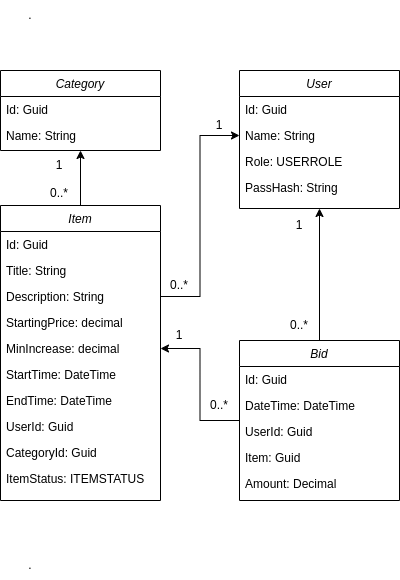
\includegraphics[scale=0.7]{daos.drawio.png}
\caption{Диаграмма моделей данных приложения и их полей}
\end{figure}

Модель User предназначена для представления информации, необходимой для аутентификации и авторизации пользователей системы. 
Она содержит уникальный идентификатор (Id), имя пользователя (Name), хеш пароля (PassHash) и роль пользователя (Role). 
Идентификатор служит для однозначной идентификации каждого пользователя, имя и хеш пароля используются для аутентификации, 
а роль определяет права доступа пользователя к различным функциям системы. 
Эта модель играет ключевую роль в обеспечении безопасности и контроля доступа к системе, 
позволяя управлять пользователями и их привилегиями.

Модель Category представляет собой сущность для хранения информации о категориях лотов в системе. 
Она содержит уникальный идентификатор (Id) категории реализованный в виде Guid, 
который позволяет однозначно идентифицировать каждую категорию, 
и Name, хранящее название категории. 
Эта модель играет ключевую роль в организации и структурировании лотов пользователей в системе, 
позволяя группировать элементы по соответствующим категориям и 
обеспечивая логическую классификацию и удобную навигацию по информации.

Модель Item представляет собой сущность, предназначенную для хранения подробной информации об элементах, 
выставляемых в системе аукциона. 
Она включает в себя уникальный идентификатор Id, 
название Title и описание Description элемента, 
начальную цену StartingPrice, минимальный шаг увеличения MinIncrease, 
даты начала StartTime и окончания EndTime аукциона, 
идентификатор пользователя UserId, выставившего элемент, 
категорию CategoryId, к которой он относится, 
а также статус элемента ItemStatus в системе аукциона. 
Эта модель обеспечивает всестороннее описание объектов, 
участвующих в коммерческих операциях системы, и служит важным элементом ее функционирования.

Модель Bid представляет собой сущность, 
которая хранит информацию о ставках, сделанных пользователями в рамках аукционных процессов системы. 
Она включает в себя уникальный идентификатор Id для каждой ставки, размер ставки Amount, 
идентификаторы пользователя UserId, сделавшего ставку, и элемента ItemId, на который была сделана ставка, 
а также дату и время DateTime, когда ставка была сделана. 
Эта модель играет ключевую роль в отслеживании и управлении ставками, 
что является основополагающим аспектом функционирования аукционных механизмов в системе, 
позволяя хранить историю торгов.


\subsection{Реализация слоя инструментов для хранения данных}

Слой инфраструктуры обеспечивает доступ приложения доступ к данным посредством реализации паттерна репозиторий, 
а также облегчает работу с репозиториями посредством реализации паттерна UnitOfWork. 
Рассмотрим классы, находящиеся на данном слое.

AppDbContext – класс, наследующийся от базового Entity Framework Core класса DbContext. 
В данном классе задается структура таблиц базы данных и проверяется существование базы данных при подключении к ней. 
В случае отсутствия необходимой базы данных, создается пустая база данных с требуемыми параметрами таблиц.
EfRepository<T> – шаблонный класс, реализующий в интерфейс IRepository, который описывается в слое приложения. 
Он имеет доступ к таблице базы данных, содержащей объекты типа T и содержит следующие методы:

– GetByIdAsync() – метод, возвращающий объект из базы данных с требуемым идентификатором. 
В случае передачи соответствующих параметров также может вместе с самим объектом вернуть объекты из других таблиц, 
связанных с ним внешними ключами;
    
– ListAllAsync() – возвращает все объекты из таблицы базы данных, связанной с данным конкретным репозиторием;
    
– ListAsync() – возвращает все объекты из таблицы базы данных, соответствующие переданному фильтру. В
 случае передачи соответствующих параметров также может вместе 
 с каждым из них вернуть объекты из других таблиц, связанных с ним внешними ключами;
    
– AddAsync() – добавляет переданный объект в базу данных;
    
– UpdateAsync() – изменяет переданный объект в базе данных;
    
– DeleteAsync() – удаляет переданный объект из базы данных;
    
– FirstOrDefaultAsync() – возвращает первый объект из базы данных, соответствующий переданному фильтру. 
В случае отсутствия такого объекта в базе данный, возвращает null.
EfUnitOfWork – класс, реализующий интерфейс IUnitOfWork, который описывается в слое бизнес-логики. 
Содержит в себе объекты класса EfRepository для каждой модели, 
а также методы CreateDataBaseAsync() и DeleteDataBaseAsync(), 
которые создают и удаляют базу данных, а также метод SaveAllAsync(), 
который сохраняет внесенные в базу данных изменения. 

\subsection{Реализация бизнес-логики}

Бизнес-логику описывают следующие интерфейсы:

– IAuthService – служит для управления авторизацией и аутентификацией пользователей. 
Он предлагает два метода: Register, который регистрирует пользователя с указанным именем пользователя и паролем, 
и SignIn, который проверяет вход пользователя с указанным именем пользователя и паролем.

– IUserService – служит для управления информацией о пользователях. 
Он предлагает три метода: GetUser, который возвращает информацию о пользователе с указанным именем пользователя, 
GetUserById, который возвращает информацию о пользователе с указанным идентификатором пользователя,
и GetUserName, который возвращает имя пользователя с указанным идентификатором пользователя.

– ICategoryService – служит для управления информацией о категориях. 
Он предлагает шесть методов: GetAll, 
который возвращает список всех категорий, GetCategory, 
который возвращает информацию о категории с указанным идентификатором категории или именем категории, 
CreateCategory, который создает новую категорию с указанным именем, ChangeCategory, 
который изменяет информацию о категории с указанным идентификатором категории, 
DeleteCategory, который удаляет категорию с указанным идентификатором, и GetCategoryName, 
который возвращает имя категории с указанным идентификатором категории.

– IItemService – служит для управления информацией о товарах. 
Он предлагает восемь методов: GetItem, 
который возвращает информацию о товаре с указанным идентификатором, GetItemsByCategory, 
который возвращает список товаров, относящихся к указанной категории, GetItemsByUserId, 
который возвращает список товаров, созданных пользователем с указанным идентификатором пользователя, 
GetItemsByUser, который возвращает список товаров, созданных пользователем с указанным именем, 
CreateItem, который создает новый товар с указанными параметрами, ChangeItemStatus, 
который изменяет статус товара, ChangeItemDetails, 
который изменяет информацию о товаре, 
и CloseItem, который закрывает товар с указанным идентификатором товара.

– IBidService – служит для управления информацией о ставках. 
Он предлагает четыре метода: GetBidsByItem, 
который возвращает список ставок, сделанных на определенный товар, 
GetBidsByUser, который возвращает список ставок, сделанных пользователем с указанным именем пользователя, 
CreateBid, который создает новую ставку с указанными параметрами, и DeleteBid, 
который удаляет ставку с указанным идентификатором ставки.


\subsection{Реализация  веб-представления}
Данный слой реализован с использованием фреймворка ASP.NET Core. 
На данном слое содержатся классы для контроллеров веб-интерфейса приложения, 
определения моделей для обмена данными с клиентом и класс для преобразования доменный моделей в DTO модели, 
класс для работы с узлом подключения к приложению для обмена данными между различными клиентами в реальном времени, 
а также точка входа в приложения. Рассмотрим отдельно каждую из этих групп классов.

Классы контроллеров веб-интерфейса приложения предоставляют публичное API (программный интерфейс приложения) 
для организации доступа к данным приложения клиентам. 
Вся внутренняя реализация методов данных классов взаимодействует только со слоем приложения, 
к каждому из них через внедрение зависимостей добавлен соответствующий сервис для решения 
определенных задач.


– AuthController – данный класс содержит в себе только два метода: 
register() и login(), которые соответственно дают доступ к регистрации и входу в аккаунт пользователя.

– UserController – отвечает за обработку запросов, связанных с пользователями, 
и использует IUserService для взаимодействия с бизнес-логикой и 
IMapper для преобразования доменных моделей в модели для предоставления данных пользователю. 

– CategoryController – управляет категориями в приложении аукциона и использует ICategoryService для взаимодействия с бизнес-логикой 
и IMapper для преобразования доменных моделей в модели для предоставления данных пользователю.

– ItemController – управляет товарами в приложении аукциона и использует IItemService для взаимодействия с бизнес-логикой, 
IHubContext для отправки сообщений в реальном времени и IMapper для преобразования доменных моделей в модели для предоставления данных пользователю.

– BidController – управляет ставками в приложении аукциона и использует IBidService для взаимодействия с бизнес-логикой, 
IHubContext для отправки сообщений в реальном времени и 
IMapper для преобразования доменных моделей в модели для предоставления данных пользователю.

Для уведомления пользователей об изменениях состояния системы аукциона используется класс AuctionHub, 
который является частью приложения аукциона и отвечает за управление соединениями клиентов и отправку сообщений в реальном времени.
Данный класс наследует класс Hub, который является частью библиотеки SignalR.

Далее рассмотрим класс преобразования доменных моделей в модели для предоставления данных пользователю. 
Данный процесс реализован с помощь библиотеки AutoMapper. 

В точке входа в приложении происходит подключение всех слоев приложения друг другу через внедрение зависимостей, 
подключение внешних зависимостей, подключение приложения к базе данный и непосредственно запуск веб-сервера. 